\documentclass[a4paper,12pt]{article}
\usepackage[utf8]{inputenc}
\usepackage[T1]{fontenc}
\usepackage[hungarian]{babel}
\usepackage{graphicx}
\usepackage{geometry}
\geometry{a4paper,
		     tmargin = 35mm, 
		     lmargin = 25mm,
		     rmargin = 30mm,
		     bmargin = 30mm}
\usepackage{mathtools}
\usepackage{amsmath}
\usepackage{color}
\usepackage{setspace}
\usepackage{amsmath,amssymb}
\usepackage{float}


\usepackage{indentfirst}
\usepackage{subfig}

\renewcommand\thesection{\Roman{section}}

\begin{document}

\linespread{1.2}

\begin{titlepage}

	\centering
	
\includegraphics[width=0.66\textwidth]{elte.jpg}\par\vspace{1cm}
	{\scshape\LARGE ELTE TTK \par}
	\vspace{3cm}
	{\scshape\Large Mössbauer-effektus vizsgálata\par}
	\vspace{1cm}
	{\large\itshape Olar Alex\par}
	\vspace{3cm}
	{\large 2018 \par}
	
\end{titlepage}

\begin{abstract}
\par A mérés célja az volt, hogy megismerkedjünk a legpontosabb energia mérési módszerrel a magfizikában, azaz a Mössbauer-effektussal. Ennek során különböző minták energiaátmeneteit vizsgáltuk, elektromos és mágneses térben.
\end{abstract}

\vfill

\tableofcontents

\newpage

\section{Elméleti összefoglaló}

\par Gerjesztett állapotó atommagok elektromágneses sugárzást bocsáthatnak ki, gamma-sugárzás formájában, amikor alacsonyabb energiaszintre kerülnek. Ennek során a kibocsátott $\gamma$-foton energiája már kisebb, mint egy ugyanilyen mag gerjesztéséhez szükséges energia, hiszen az anyamag visszalökődik. Ahhoz, hogy a kibocsátott foton újra gerjeszteni tudjun a természetes vonalszélességét (energiájának bizonytalanságát) kell növelni. A labor során használt módszer egy hangfalhoz kötötte a mintákat, amiket az állandó gyorsulással rezgetett. A fotonok Doppler-effektusa okozta a vonalkiszélesedést. Így a fotonok már újra el tudtak nyelődni. Az anyagok vizsgálata során elektromos és mágneses térbe is helyezzük a mintákat, vizsgálva például ezáltal a Zeemann-felhasadást.

\vspace{5mm}

\par A Doppler-effektus a sebességgel arányos

\begin{equation*}
	\Delta E = E\sqrt{\frac{c+v}{c-v}} - E \approx E\frac{v}{c}
\end{equation*}

\par Azaz a sebességgel arányos a vonalkiszélesedés. A mérés egy sokcsatornás analizátorra van kötve, amely pedig egy proporcionális kamráról kapja az impulzusokat. Ez az $^{57}Co$ $14.4~keV$-es $\gamma$-fotonjaira érzékeny, amivel a mintát besugározzuk. A mérési berendezés része egy diszkriminátor is, amely a kisebb és nagyobb energiájú fotonokat nem engedi a sok csatornás analizátorra. A spektrum mérése számítógéppel történt a különböző minták behelyezése után.

\section{Mérési eszközök}

\begin{itemize}
\item sokcsatornás anlizátor kártya
\item számítógép
\item diszkriminátor
\item $^{57}Co$, valamint $\text{nátriumprusszid}$,
$\text{lágyvas}$ és $\text{rozsdamentes-acél}$ minták
\end{itemize}

\section{A mérés menete}

\par Először a diszkriminátort állítottuk a megfelelő tartományba, hogy ténylegesen csak a $14.4~keV$-es fotonokat észleljük. A lineáris csatornaszám, energia kalibráláshoz a lágyvas minta Mössbauer-sprektrumát hasznátluk fel.

\subsection{Kalibrálás}

\par A két legszélső csúcs közötti távolság, Doppler-sebességben adott volt, $d_{v} = 10.6162 \frac{mm}{s}$, míg a csúcsok távolságát Lorentz-gröbék illesztésével nyertük. Az illesztés és a kalibrálás értéke

\begin{figure}[!htb]
\centering
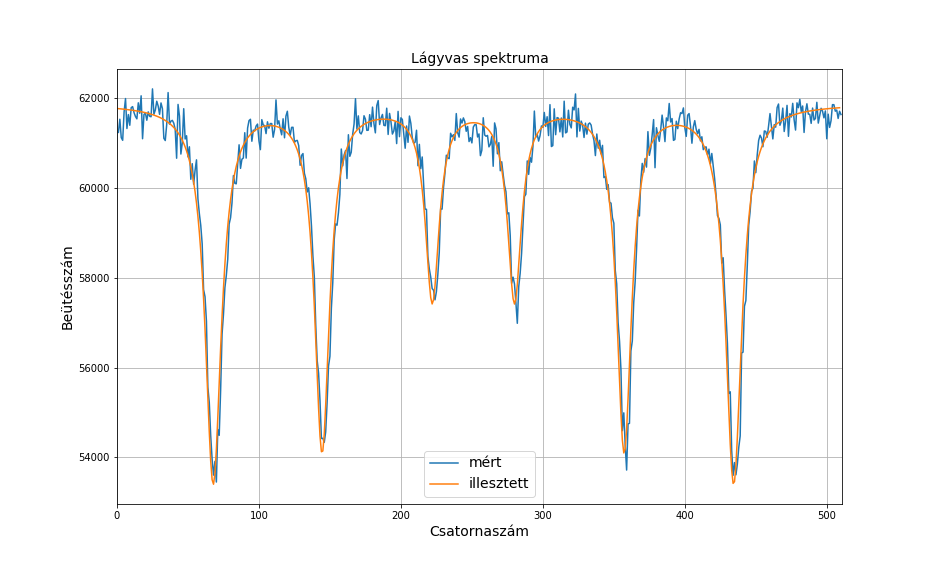
\includegraphics[width=0.75\textwidth]{vas.png}
\caption{A lágyvas sprektruma és a rá illesztett Lorentz-görbék}
\end{figure}

\par Innen leolvasható, hogy a két szélső csúcs távolsága $d_{ch} = 366.6 \pm 0.1$ csatornaszámban megadva. Ebből számolható a az energia-csatorna átvátálsi tényező (ezután $\Delta^{*}$)

\begin{table}[h]
	\begin{center}
	\begin{tabular}{|l|c|}
		\hline
		\textbf{paraméter} & \textbf{illesztett érték} \\
		\hline
		\multicolumn{2}{c}{Lágyvas} \\
		\hline
		alapvonal ($B$) & $61883 \pm 22 $\\
		\hline
		1. amplitúdó ($A_1$) & $8418 \pm 83 $\\
		\hline
		1. csúcs helye (felhasadás nélkül) ($x_{0, 1}$) & $252.09 \pm 0.07$\\
		\hline
		1. csúcs szélessége ($\Gamma_1$) & $13.86 \pm 0.2$\\
		\hline
		1. felhasadás ($S_1$) & $366.6 \pm 0.1$ \\
		\hline
		2. amplitúdó ($A_2$) & $7682 \pm 86 $\\
		\hline
		2. csúcs helye (felhasadás nélkül) ($x_{0, 2}$) & $251.86\pm 0.07$\\
		\hline
		2. csúcs szélessége ($\Gamma_2$) & $12.62 \pm 0.2 $\\
		\hline
		2. felhasadás ($S_2$) & $212.8 \pm 0.1$ \\
		\hline
		3. amplitúdó ($A_3$) & $4327 \pm 89 $\\
		\hline
		3. csúcs helye (felhasadás nélkül) ($x_{0, 3}$) & $252.06 \pm 0.12$\\
		\hline
		3. csúcs szélessége ($\Gamma_3$) & $11.89 \pm 0.4$\\
		\hline
		3. felhasadás ($S_3$) & $57.92 \pm 0.24$ \\
		\hline
	\end{tabular}
	\end{center}
	\caption{Illesztett görbe paraméterei}
	\label{tab:params}
\end{table}


\begin{equation*}
	\Delta^{*} = E_{\Gamma}\frac{d_{v}}{d_{ch}\cdot c} = (1.3909 \pm 0.0005) \cdot 10^{-9} eV
\end{equation*}

\par Azaz megkaptuk a Doppler-effektusból származó energiakiszélesedés értékét csatornaszámra vonatkoztatva.

\subsection{Energia-eltolódás a lágyváshoz képest}

\par Ehhez meg kellett határozni a nem felhasadt csúcs helyét mindhárom esetben, ehhez a további két spektrumot is illeszteni kellett és mivel 6 kölönböző csúcs volt a lágyvasnál, 3 különböző középértékkel, így azokat átlagoltuk.

\par Az illesztések paraméterei pedig

\begin{table}[!htb]
	\begin{center}
	\begin{tabular}{|l|c|}
		\hline
		\textbf{paraméter} & \textbf{illesztett érték} \\
		\hline

		\hline
		\multicolumn{2}{c}{Rozsdamentes acél} \\
		\hline
		alapvonal ($B$) & $1170.6 \pm 1.7 $\\
		\hline
		amplitúdó ($A$) & $342.0 \pm 13.3 $\\
		\hline
		csúcs helye ($x_0$) & $247.65 \pm 0.32$\\
		\hline
		szélesség ($\Gamma$) & $16.57 \pm 0.96$\\
		\hline

		\hline
		\multicolumn{2}{c}{Nitroprusszid-nátrium} \\
		\hline
		alapvonal ($B$) & $2631.9 \pm 2.6 $\\
		\hline
		amplitúdó ($A$) & $364.5 \pm 18.7 $\\
		\hline
		csúcs helye (felhasadás nélkül) ($x_0$) & $242.55 \pm 0.25$\\
		\hline
		szélesség ($\Gamma$) & $9.86 \pm 0.73$\\
		\hline
		felhasadás ($S$) & $59.51 \pm 0.50$ \\
		\hline

	\end{tabular}
	\end{center}
	\caption{A további illesztett görbék paraméterei}
	\label{tab:params2}
\end{table}

\begin{figure}[!htb]
    \centering
    \begin{minipage}{.49\textwidth}
        \centering
        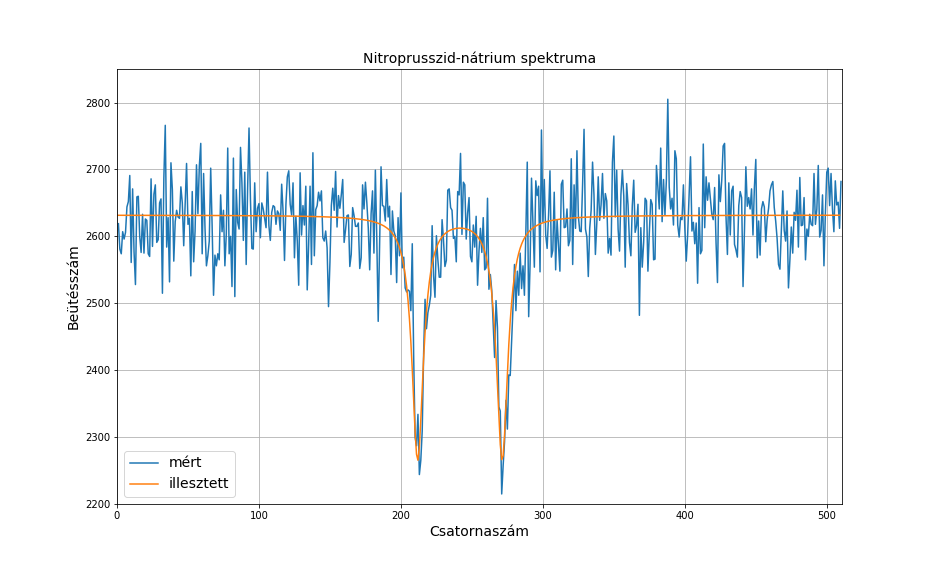
\includegraphics[width=1.\linewidth]{np.png}
        \caption{A nitroprusszid sprektruma és a rá illesztett Lorentz-görbék}
    \end{minipage}
    \begin{minipage}{.49\textwidth}
        \centering
        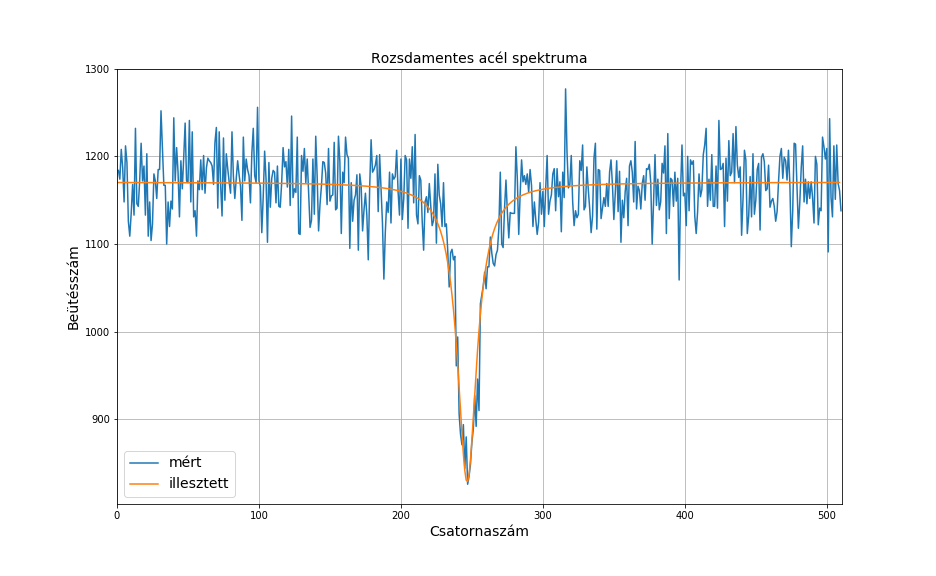
\includegraphics[width=1.\linewidth]{acel.png}
        \caption{Az acél sprektruma és a rá illesztett Lorentz-görbe}
    \end{minipage}
\end{figure}

\begin{table}[!h]
\begin{center}
\begin{tabular}{|c|c|c|}
\hline
 & csúcs helye & abszolút hiba \\
\hline
lágyvas & 252.003 & 0.157 \\
\hline
nitroprusszid & 242.555 & 0.252 \\
\hline
acél & 247.648 & 0.322 \\
\hline
\end{tabular}
\end{center}
\caption{A csúcsok helyei és azok hibái}
\end{table}

\pagebreak

\par Ebből az előbbi $\Delta^{*}$ paraméterrel számolható a vas-acél és vas-nitroprusszid eltolódás

\begin{table}[!htb]
\begin{center}
\begin{tabular}{|c|c|c|}
\hline
 & ernegia [$10^{-9}$ eV] & abszolút hiba [$10^{-9}$ eV] \\
\hline
lágyvas-acél & 6.0579 & 0.4999 \\
\hline
lágyvas-nitroprusszid & 13.1418 & 0.4182 \\
\hline
\end{tabular}
\end{center}
\caption{Izomér eltolódás}
\end{table}

\par Az energia értékekhez a lágyvascsúcshoz képesti csatornaszámkülönbségét ($\Delta_{ch}$) és az előbb számított $\Delta^{*}$-t használtuk

\begin{equation*}
 \Delta E = \Delta^{*}\cdot \Delta_{ch}
\end{equation*}

\subsection{A gerjesztett állapotok élettartama}

\par A lágyvas 6 részre hasadt csúcsainak vonalszélességéit az illeszétsekből korábban magkaptuk. Az intenzitásuk a csúcsok alatti területtel arányos. A mért vonalszélesség, intezitás és valós vonalszélessgé között a következő összefüggés ismert

\begin{equation*}
	\Gamma_{\text{mért}}^{(i)} = 2.405\Gamma + \frac{1}{4}w_{i}T_{A}\Gamma
\end{equation*}

\par Amely egyenletben $w_{i}$ a számolt intenzitások, $T_{A}$ a minta vastagsága, és elhanyagolásokat eszközültünk.

\begin{center}
\begin{tabular}{|c|c|c|}
\hline
Intenzitás & $\Gamma_{\text{mért}}^{(i)}$ [$10^{-9}$ eV] & $\Gamma_{\text{mért}}^{(i)}$ hiba [$10^{-9}$ eV] \\
\hline
0.22 & 19.2958 & 0.278 \\
\hline
0.183 & 17.5695 & 0.278 \\
\hline
0.097 & 16.5532 & 0.5574\\
\hline
\end{tabular}
\end{center}

\par Ezekre az adatokra egyenest illesztve, annak $\Gamma_{\text{mért}}^{(i)}$ tengellyel vett metszete adja majd $2.4\cdot\Gamma$-t, azaz a valódi vonalszélesség értékét. Ezt eszközölve

\begin{figure}[!htb]
\centering
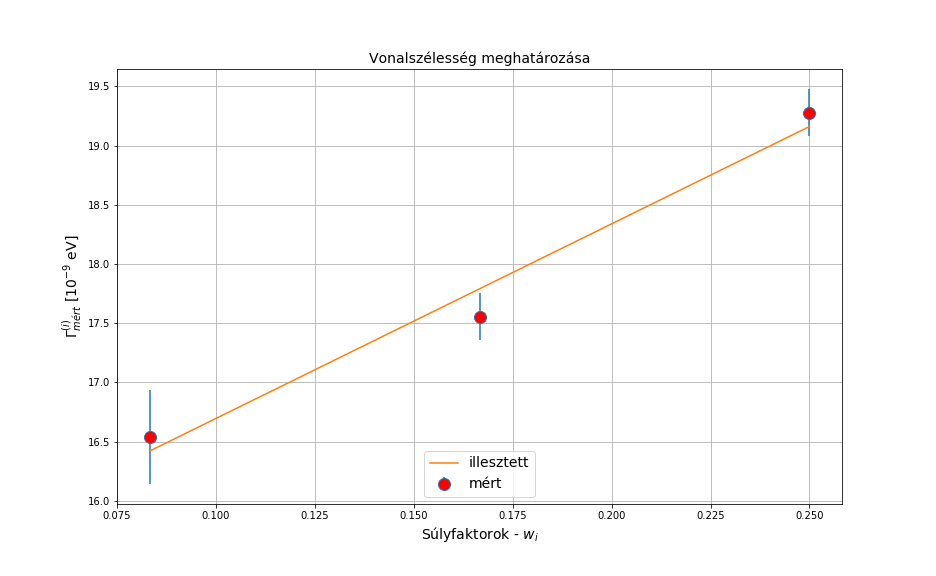
\includegraphics[width=0.55\textwidth]{vonalszelesseg.png}
\caption{A vonalszélesség vizsgálata}
\end{figure}

\par Az illesztett egyenes adatai pedig

\begin{equation*}
\Gamma_{\text{mért}}(I) = 2.405\Gamma + \frac{1}{4}IT_{A}\Gamma = (13.607 \pm 2.283)\cdot 10^{-9} + (24.312 \pm 11.799)\Gamma eV
\end{equation*}

\par Azaz ebből kapjuk, hogy a vonalszélesség valós értéke

\begin{equation*}
	\Gamma = (5.658 \pm 0.949)\cdot 10^{-9} ~eV
\end{equation*}

\par Innen már könnyen számaztatható az átlagos élettartam ami $\Gamma = \frac{\hbar}{\tau}$-ból számolható

\begin{equation*}
	\tau = (116.34 \pm 19.52) ~ns
\end{equation*}

\par Ez az irodalmi adattól még hibahatáron belül is több mint $5\%$-al eltér. Ennek okát nem tudjuk, csak találgatni tudunk, hiszen az illesztésünkön is pontosítottunk ameddig csak lehetett.

\subsection{Elektromos térgradiens a nitroprusszid mintában}

\par A nátrium-nitroprusszidban az atomok elrendeződése miatt inhomogén elektromos tér alakul ki, ami kölcsönhat a mag kvadrupólmomentumával így az enrgiaszintek az alábbi egyenlet szerint felhasadnak

\begin{equation*}
\Delta E = \frac{eQ}{4I(2I - 1)}\frac{\partial^{2}V}{\partial z^{2}}(3m_{I}^{2} - I(I+1))\sqrt{1+\frac{\eta^{2}}{3}}
\end{equation*}

\par A kvadrupólmomentum, Q, adott $0.21\cdot 10^{-28} m^{2}$, míg I = 3/2, valamint $\eta = 0$. A megfeleleő értékeket behelyettesítve azt vehetjük észre, hogy csak két részre hasadnak az energia-szintek

\begin{equation*}
\Delta E = \frac{eQ}{2}\frac{\partial^{2} V}{\partial z^{2}}
\end{equation*}

\par A kiszélesedés energiaértékét ki tudjuk számolni a korábbi $\Delta^{*}$ paraméterrel. A többi adat adott, így a térgradiens értéke

\begin{equation*}
\frac{\partial^{2}V}{\partial z^{2}} = (7.883 \pm 0.0697) \cdot 10^{21} ~\frac{V}{m^{2}}
\end{equation*}

\par Elméleti úton kapjuk, hogy a Bohr-modellben a proton helyén, a Coulomb-potenciál kétszeri deriválásával kapjuk, hogy

\begin{equation*}
\frac{\partial^{2}V}{\partial z^{2}} = 1.95 \cdot 10^{22} ~\frac{V}{m^{2}}
\end{equation*}

\par Azaz közel 1 nagyságrendet tévedtünk, de egészen jól megközelítettük a Bohr-modellben prezentált elméleti értéket.

\subsection{Az $^{57}Fe$ vas mágneses momentuma, másneses térbeli felhasadás}

\par A mágneses knvatumszámok szerinti felhasadást a Zeemann-effektus írja le. Az energiaeltolódást az $m$ kvantumszám szerint a következő összefüggés adja meg

\begin{equation*}
	\Delta E_{m} = -\frac{m_{I}}{I}\mu_{I}B
\end{equation*}

\par A vizsgált minta energiaszintjei 6 részre hasadnak, amelyek között hat átmenet lehetséges. Az $I = 3/2$ és $I = 1/2$ enegiaszintek közötti energia különbség $\Delta E_{I}$, míg ezek közül a nagyobb 4, míg a kisebb magspinű 2 részre hasad. Az utóbbi energiakülönbsége $\Delta E_{1/2}$, míg az előbbié az egymás mellettiek között $\Delta E_{3/2}$. Így Az átmenetekhez tartozó energiakülönségek táblázatba foglalva

\begin{table}[h!]
\centering
\begin{tabular}{|c| c|} \hline
Ámenet& Energia értékek paraméterekkel \\ \hline
$\pm \frac{3}{2}\leftarrow\pm\frac{1}{2}$& $\Delta E_{1/2}$+3$\Delta E_{I}$\\ \hline
$\pm \frac{1}{2}\leftarrow\pm\frac{1}{2}$& $\Delta E_{1/2}$+$\Delta E_{I}$\\ \hline
$\pm \frac{3}{2}\leftarrow\mp\frac{1}{2}$& $\Delta E_{1/2}$-$\Delta E_{I}$\\ \hline
\end{tabular}
\caption{Energia-átmenetek}
\end{table}

\par Innen $ N = C\cdot \Delta E + A$ egyenesre illesztést végeztünk, ahol $\Delta E$ az előbbi táblázat második oszlopában lévő energiaadatok, melyek értéke

\begin{table}[h!]
\centering
\begin{tabular}{|c |c|} \hline
Átmenet & Energiaszint($10^{-9}~eV$)\\ \hline
$\Delta E_1$ & $509.9\pm0.19$\\ \hline
$\Delta E_2$ &  $295.98\pm0.16$\\ \hline
$\Delta E_3$ & $80.56\pm0.33$\\ \hline
\end{tabular}
\end{table}

\par Majd az illesztés

\begin{figure}[h!]
\centering
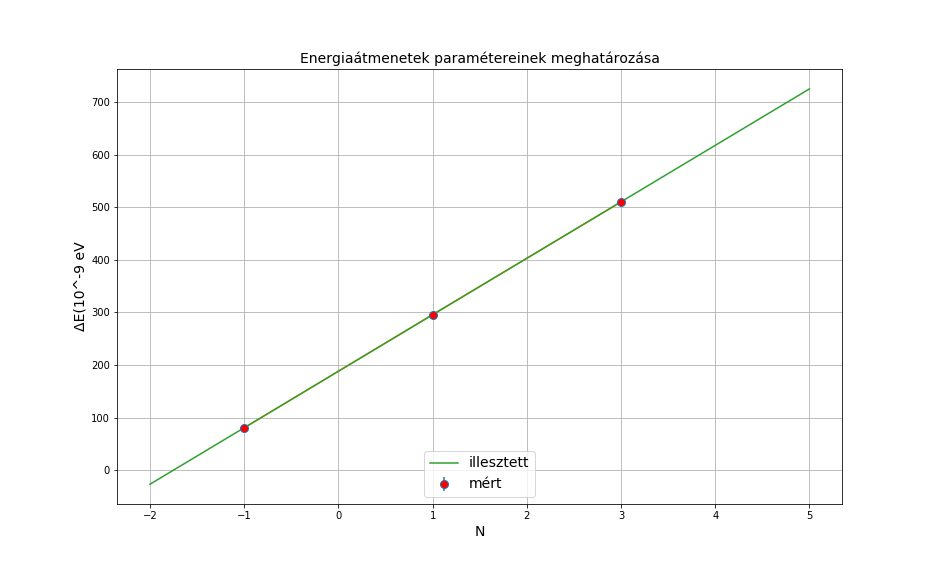
\includegraphics[width=0.55\textwidth]{parameterek.png}
\caption{Zeemann-felhasadás, a mágneses momentum származtatható}
\end{figure}

\par Tudjuk, hogy alapállapotban $\mu_{1/2} = 0.090604\cdot \mu_{N}$, valamint 

\begin{equation*}
\Delta E = \frac{\mu_{1/2}B}{I_{1/2}} = A \quad \quad \Delta E = \frac{\mu_{3/2}B}{I_{3/2}} = -C 
\end{equation*}

\par Ahol $A$ és $C$ az illesztés paraméterei

\begin{table}[!h]
\centering
\begin{tabular}{|c|c|} \hline
A [$10^{-9}~eV$] & B [$10^{-9}~eV$] \\ \hline
(188.145 $\pm$ 0.414) & (107.335 $\pm$ 0.216) \\ \hline
\end{tabular}
\end{table}

\par Ebből $\mu_{3/2}$ egy osztás után meghatározható, majd B is számolható

\begin{equation*}
\mu_{3/2} = (-5.43 \pm 0.13) \cdot 10^{-9} ~\frac{eV}{T} \quad \quad B = (32.94 \pm 0.07) ~T
\end{equation*}

\par Az elméleti érték a Bohr-modell alapján kapható, amihez képest a mért adat közel háromszoros.

\begin{equation*}
B_{\text{elméleti}} = \frac{\mu_{0}\hbar c}{m_{e}4\pi r_{Bohr}^{2}} \approx 12.5 ~T
\end{equation*}

\section{Lehetséges hibák, gravitációs vöröseltolódás}

\par A mérés során az állandónak vett minta-forrás távolság természetesen változik, hiszen pontosan a minta mozgatása miatti Doppler-effektus szélesíti ki az energianívókat. A háromszögjel periódusideje a jegyzet szerint $T = 41.2 \pm 2 ~ms$, a maximális sebesség pedig

\begin{equation*}
v_{max} = c \frac{\Delta E_{\text{szélső}}}{E_{0}} = (7.418 \pm 0.002) ~\frac{mm}{s}
\end{equation*}

\par Ahol $E_{szélső}$ a legutolsó 255-ös csatorna energiaszintjéhez tartozó kiszélesedés. A maximális kitérés így $v_{max}\frac{T}{4}$, hiszen a periódusidő negyedénél van maximuma a sebsségnek

\begin{equation*}
d_{max} = (0.0764 \pm 0.004) ~mm
\end{equation*}

\subsection{Gravitációs vöröseltolódás}

\par A Föld felszín közeli gravitációs potenciálja $\varphi = gh$. A laborban $0.5$ csatorna pontossággal tudunk mérni ez azt jelenti, hogy a kezdeti $\Delta^{*}$ energia fele lehet a mérés hibája, hogy meg tudjuk határozni a gravitációs vöröseltolódást, amit a potenciálkülönbség miatt szenved el a fény. Így

\begin{equation*}
h = \frac{\Delta^{*}}{2\cdot E_{\Gamma}}\frac{c^{2}}{g} \approx 440 ~m
\end{equation*}

\par Ahol $E_{\Gamma}$ a mérésben használt $14.4 ~keV$-es foton energiája. Jól látható, hogy annak ellenére, hogy ezt a '60-as években kimérték, mi nem tudnánk ilyen $\Gamma$-fotonokkal reprodukálni.

\section{Összefoglalás}

\par Ez volt eddig a legnehezebb mérésünk. Kicsit talán sok kiértékelési feladat van, és a feladatok leírásából nem egyszerű rájönni, hogy pontosan hogyan kell végrehajtani a kiértékelést, de általánosságban természetesen nem túl bonyolult feladatokat kaptunk. A hibákat végig hibaterjedéssel számoltuk, a feladatokat közösen értékeltük ki, így az ábráink és néhol a táblázataink megegyezhetnek. Összességében sikeres mérést kiviteleztünk.

\end{document}